


\setlength{\columnsep}{15pt}%
\setlength{\intextsep}{0pt plus 0pt minus 0pt}


\setlength{\parindent}{\myindent}
% \setlength{\parskip}{\myparskip}

    \mybox{
    I wish to earn my Ph.D. in the field of computer vision. My interest lie in the field of computer vision and machine learning (ML), with a focus on perception and scene understanding. I am particularly interested in self-supervised and semi-supervised learning techniques, as they are crucial for real-world applications with limited data annotation. In my previous research, conducted at the Research Center for Information Technology (FZI) under the guidance of Dr. Ömer Sahin Tas and in the context of my master’s thesis under the supervison of Prof. Christoph Stiller, I worked on self-supervised learning using masked image modelling, 2D and 3D object detection on camera and LiDAR input, and multimodal fusion. I am keen to engage in independent research while working in collaborating with fellow researchers to exchange ideas and insights. I am also interested in mentoring students and assisting them with their research projects.}
    
    \subsection{\textbf{Background}} \begin{wrapfigure}{r}{110pt}
        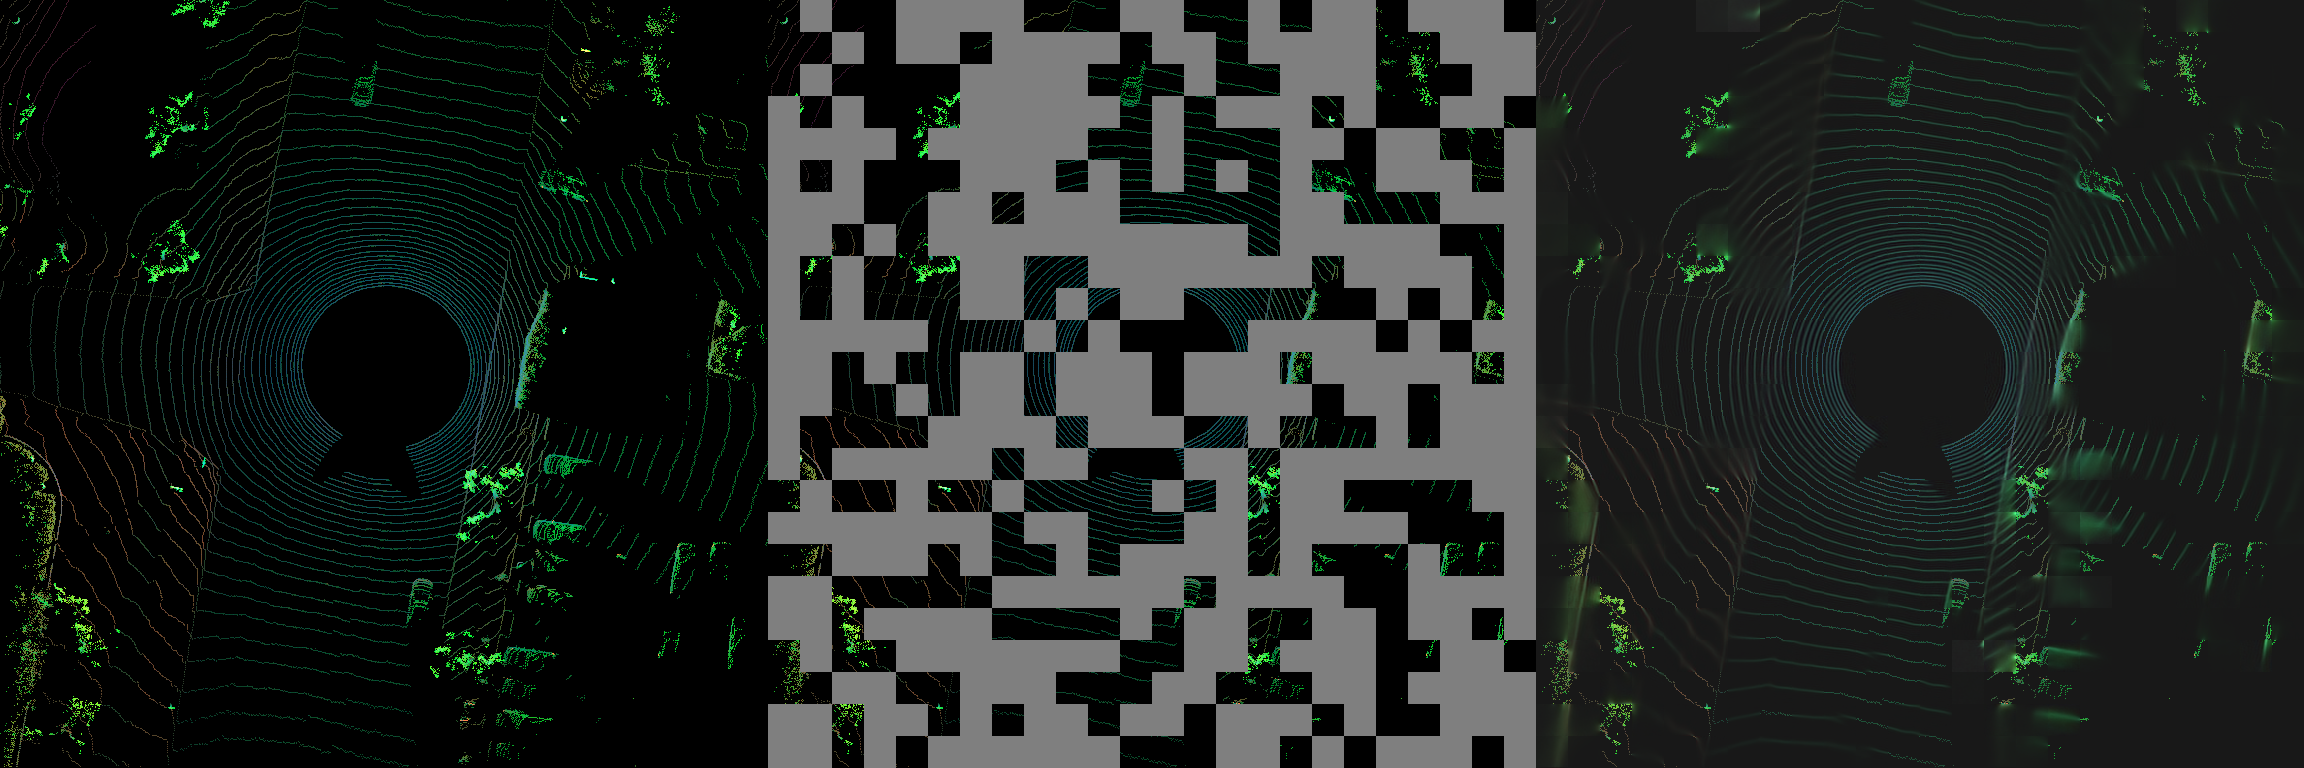
\includegraphics[width=330pt, angle=270]{pic/Hiera-Waymo.png}
        \mainfont\fontsize{9pt}{9pt}\selectfont\caption{ \mainfont\fontsize{9pt}{9pt}\selectfont Masked Autoencoding 
        (MAE) of Bird's Eye View Point Cloud Representation on Waymo Open Perception Dataset. From top to bottom: Input, Masked, Reconstruction}
        \label{fig:mae_img}
        \end{wrapfigure}
    
    During my Bachelor's degree at the Karlsruhe Institute of Technology (KIT), I focused my studies in computational mechanics. This enabled me to develop a comprehensive understanding of tensor algebra, tensor analysis and optimisation. In my Bachelor's thesis, supervised by Prof. Thomas Böhlke, I conducted research into algorithms for generating higher-order irreducible tensor representations in the context of mechanical texture development. I explored the field of computer vision and machine learning through the exceptional course on machine vision taught by Dr. Martin Lauer. It was immediately apparent that the mathematical methods employed in continuum mechanics were highly transferable, which inspired me to pursue a career in this field.

    Motivated by the course on Machine Vision I applied for the internship at SICK AG, where I contributed to the embedded application layer of a smart 3D-ToF camera. The camera is used to detect obstacles on mobile agents within indoor environments using classical ML methods. In discussions with colleagues, it was determined that the lack of labelled point cloud data were the main reason for the slow implementation of deep learning, further emphazising the importance of self-supervised and unsupervised learning techniques. During my internship and period as a working student, I developed my skills as a software engineer and became a more effective team player through hands-on experience and collaboration.

    As part of my Information Technology major field, I had the opportunity to participate in the Data Driven Engineering I/II course series by Dr. Cihan Ates, where I built a strong foundation in machine learning. In the context of my research project, entitled "Energy Consumption Prediction at High Granularity", I competed at the lecture accompanying project contest, where I was placed in the top three. I gained valuable experience in the practical application of  both classical regression and forecasting methods and recurrent neural network approaches. In the second Data Driven Engineering course, my team and I worked on particle velocity and uncertainty estimation using convolutional autoencoders based on a variance attenuation loss. 


